\documentclass{article}
\usepackage[utf8]{inputenc}
\usepackage[UTF8]{ctex}
\usepackage{amssymb}
\usepackage{amsmath}
\usepackage{fancyhdr}
\usepackage{a4wide}
\usepackage{listings}
\usepackage{graphicx}
\usepackage{float}
\usepackage{booktabs}%第二个包定义了几个*rule
%___________________________package__________________________________%


\title{\vspace{-1\baselineskip}
\huge{\textbf{Fastjson 项目报告}}
}
\author{LiHanxuan \qquad Student number: 2017K8009908009 \\{\tt lihanxaun17@mails.ucas.ac.cn}}
\date{January 2020}

\fancypagestyle{plain}{%
\fancyhf{}
\fancyhead[LO,RE]{\sffamily University of Chinese Academy of Science}
\fancyhead[RO,LE]{\sffamily OBJECT-ORIENTED PROGRAMMING}
\fancyfoot[LO,RE]{\sffamily /Computer Science}
\fancyfoot[RO,LE]{\sffamily\bfseries\thepage}
\renewcommand{\headrulewidth}{0pt}
\renewcommand{\footrulewidth}{0pt}
}

\pagestyle{fancy}
\fancyhf{}
\fancyhead[RO,LE]{\sffamily University of Chinese Academy of Science}
\fancyhead[LO,RE]{\sffamily OBJECT-ORIENTED PROGRAMMING}
\fancyfoot[LO,RE]{\sffamily /Computer Science}
\fancyfoot[RO,LE]{\sffamily\bfseries\thepage}
\renewcommand{\headrulewidth}{1pt}
\renewcommand{\footrulewidth}{0pt}


\begin{document}
\maketitle


\section*{\Large 一、Fastjson简介及反序列化功能的建模}
\subsection*{1. JSON介绍}
\subsubsection*{1.1 JSON背景}
JSON是 JavaScript 的一个严格的子集,利用了 JavaScript 中的一些模式来表示结构化数据,用来作为一种轻量级的数据交换格式,作用类似于XML。它不是一种编程语言,仅用来描述数据结构。Douglas Crockford在2001年开始推广JSON数据格式,在2005年-2006年正式成为主流的数据格式,雅虎和谷歌就在那时候开始广泛地使用JSON格式。

\begin{figure}[htp]
\centering % 图片居中
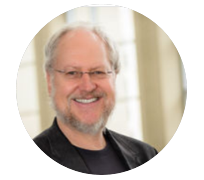
\includegraphics[width = 4cm]{pic1.png}
\caption{Douglas Crockford}
\end{figure}

\subsubsection*{1.2 JSON语法}
\begin{figure}[H]
\centering % 图片居中
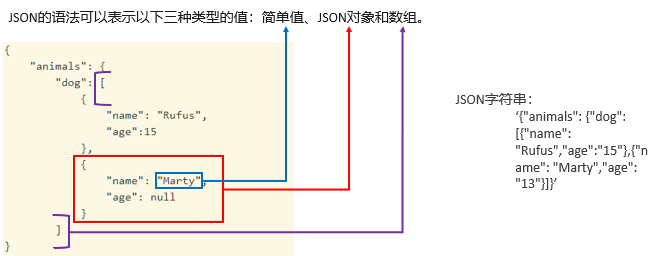
\includegraphics[width = 15cm]{pic2.png}
\end{figure}


\subsubsection*{1.2 JSON优点}
JSON的作用类似于XML,实际上JSON也就是为了取代XML而诞生的,因此再也没有比用XML与其做对比更好的方式来说明JSON的优越性了。下面简单地举一个例子来说明JSON更加简洁、轻量、可读的优点。
\begin{figure}[htb]
\centering % 图片居中
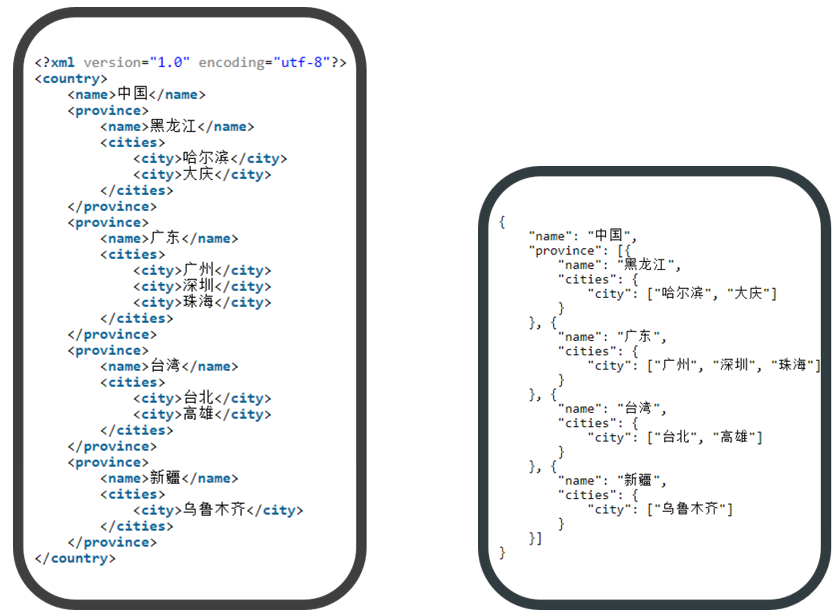
\includegraphics[width = 17cm]{pic3.png}
\caption{XML vs JSON}
\end{figure}


以上从左到右分别为具有相同含义的XML和JSON代码,可以明显地看出JSON的语法要更加简洁轻量、且更接近人类阅读的习惯。


\subsection*{2. Fastjson介绍}
\subsubsection*{2.1 Fastjson功能及优点}
对于Fastjsoon,阿里官方给的定义是, Fastjson 是阿里巴巴的开源JSON解析库,它可以解析 JSON 格式的字符串,支持将 Java Bean 序列化为 JSON 字符串,也可以从 JSON 字符串反序列化到 JavaBean。其核心功能如下图所示:
\begin{figure}[H]
\centering % 图片居中
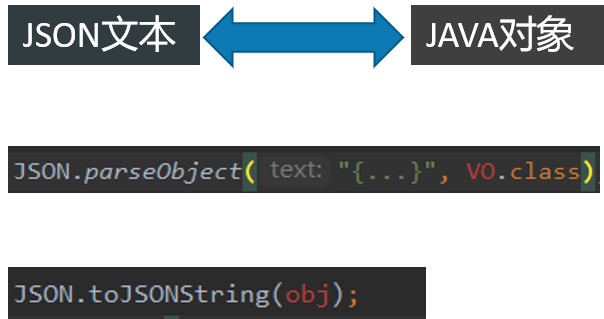
\includegraphics[width = 6cm]{pic4.png}
\caption{Core Function of Fastjson}
\end{figure}
Fastjson的优点为:
\begin{itemize}%项目符号开始
\item 速度快:fastjson相对其他JSON库的特点是快,从2011年fastjson发布1.1.x版本之后,其性能从未被其他Java实现的JSON库超越。
\item 使用广泛:fastjson在阿里巴巴大规模使用,在数万台服务器上部署,fastjson在业界被广泛接受。在2012年被开源中国评选为最受欢迎的国产开源软件之一。
\item 测试完备:fastjson有非常多的testcase,在1.2.11版本中,testcase超过3321 个。每次发布都会进行回归测试,保证质量稳定。
\item 使用简单:fastjson的 API 十分简洁。
\item 功能完备:支持泛型,支持流处理超大文本,支持枚举,支持序列化和反序列化扩展。
\end{itemize}


\subsubsection*{2.2	Fastjson调用}
\begin{figure}[H]
\centering % 图片居中
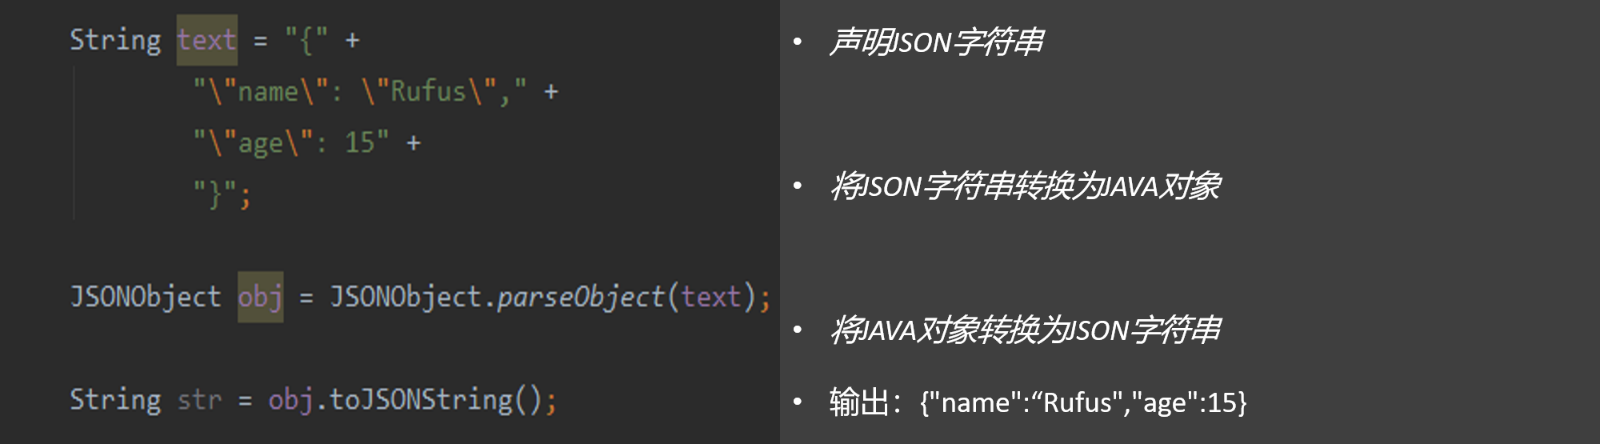
\includegraphics[width =18cm]{pic5.png}
\caption{An Example of Fastjson}
\end{figure}

\subsubsection*{2.3	Fastjson应用场景}
\begin{itemize}
\item Web框架处理JSON参数返回JSON结果
\item 远程方法调用RPC
\item Android/阿里云手机处理JSON
\item MessageQueue 传输对象
\item 配置文件代替XML
\item 保存数据到磁盘、数据库、Hbase
\end{itemize}

\subsubsection*{2.4	Fastjson开发者}
\begin{figure}[H]
\centering % 图片居中
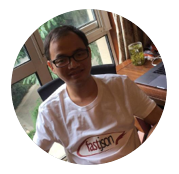
\includegraphics[width = 4cm]{pic6_1.png}
\caption{温绍锦, 阿里巴巴集团高级专家,Druid和Fastjson开源项目的主要开发者}
\end{figure}
\begin{figure}[H]
\centering % 图片居中
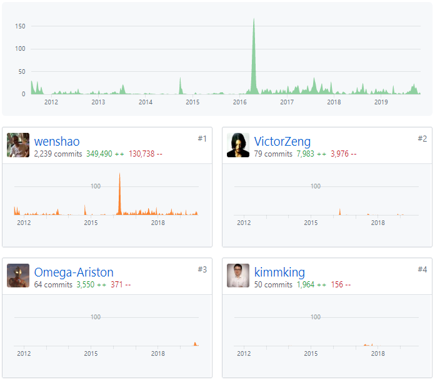
\includegraphics[width = 13cm]{pic6_2.png}
\caption{Fastjson贡献排行}
\end{figure}

\subsection*{3. 反序列化功能的需求分析}
\noindent \rule{\textwidth}{0.7mm}
下面对反序列化过程面向需求建模,反序列化过程的目的是将JSON文本转化为JAVA对象。
\begin{itemize}
\item 输入:JSON文本
\item 调用解析器进行处理
\item 返回:JAVA对象
\end{itemize}
反序列化过程的约束与限制是:
\begin{itemize}
\item 能够自行判断输入是否合理
\end{itemize}
\rule{\textwidth}{0.7mm}
按照上述需求,建立三个类:解析器Parser、扫描分析器Scanner、JAVA对象
\begin{figure}[H]
\centering % 图片居中
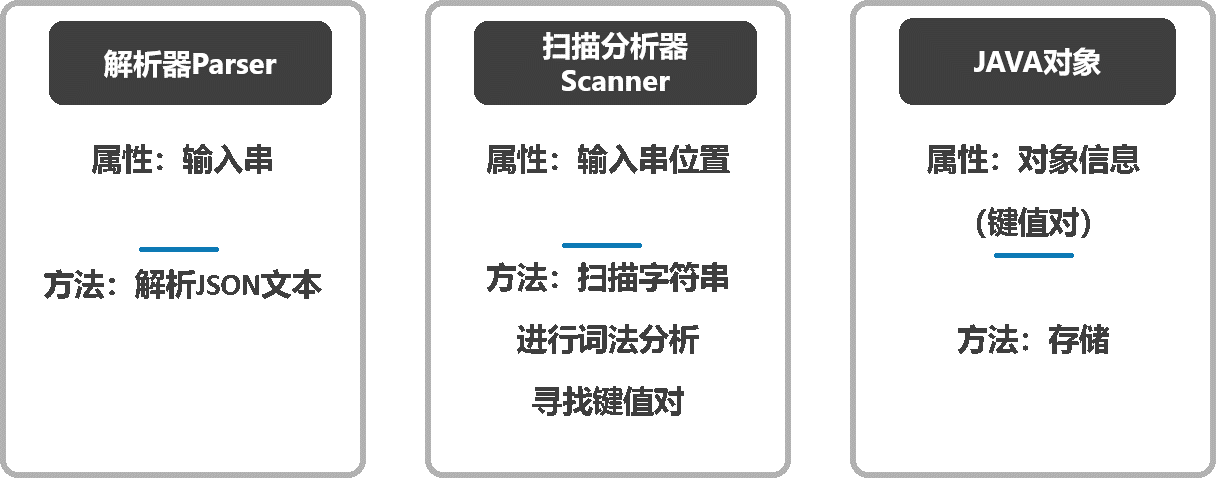
\includegraphics[width = 11cm]{pic7.png}
\caption{Class Diagram}
\end{figure}

按照该建模对整个反序列化场景进行描述如下图所示:
\begin{figure}[H]
\centering % 图片居中
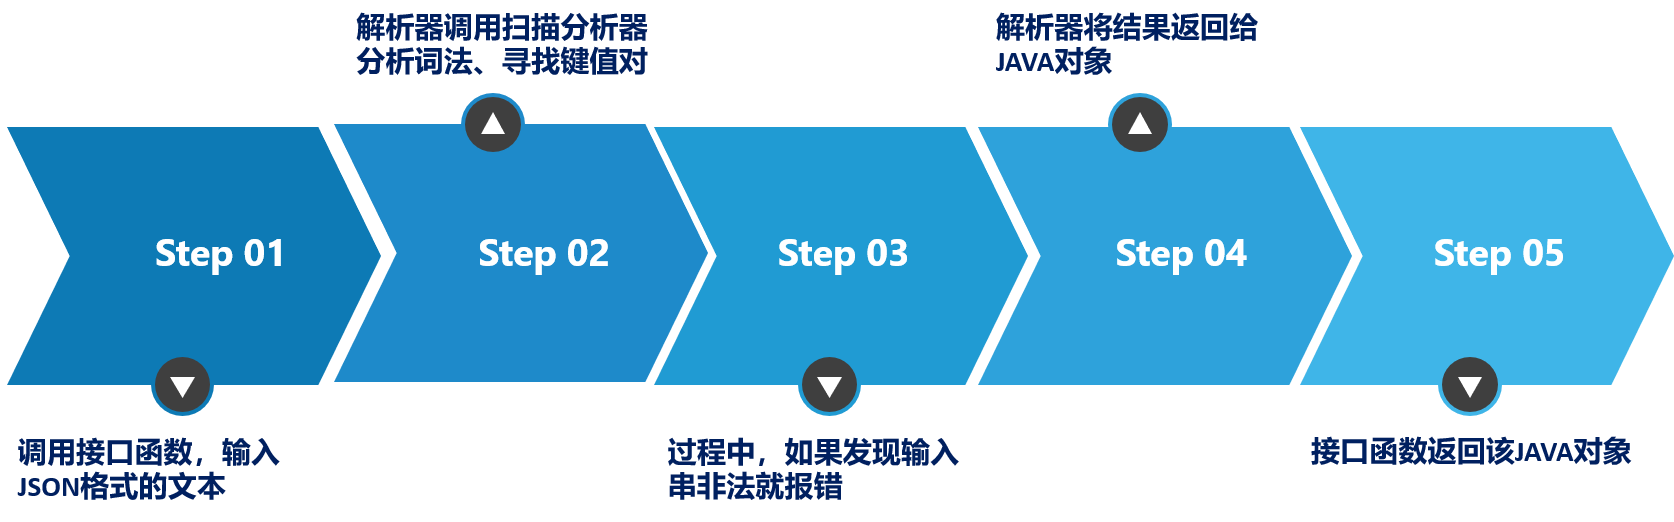
\includegraphics[width = 15cm]{pic8.png}
\caption{Flow Chart}
\end{figure}
\begin{itemize}
\item Step1:调用接口函数,输入JSON格式的文本
\item Step2:解析器调用扫描分析器分析词法、寻找键值对
\item Step3:过程中如果发现输入串非法就报错
\item Step4:解析器将结果返回给JAVA对象
\item Step5:接口函数返回该JAVA对象
\end{itemize}

\section*{\Large 二、核心流程的设计分析}
\subsection*{1. 核心流程解析}
回顾上节描述的反序列化流程,在DEBUG模式中对该流程进行追踪,并依据各类依赖性关系图进行定位:\\
\rule{\textwidth}{0.7mm}
\begin{itemize}
\item 解析器Parser:		DefaultJSONParser
\item 扫描分析器Scanner:    JSONScanner
\item JAVA对象:			    JSONObject
\end{itemize}
\rule{\textwidth}{0.7mm}

Step1: 调用接口函数,输入JSON格式的文本
\begin{figure}[H]
\centering % 图片居中
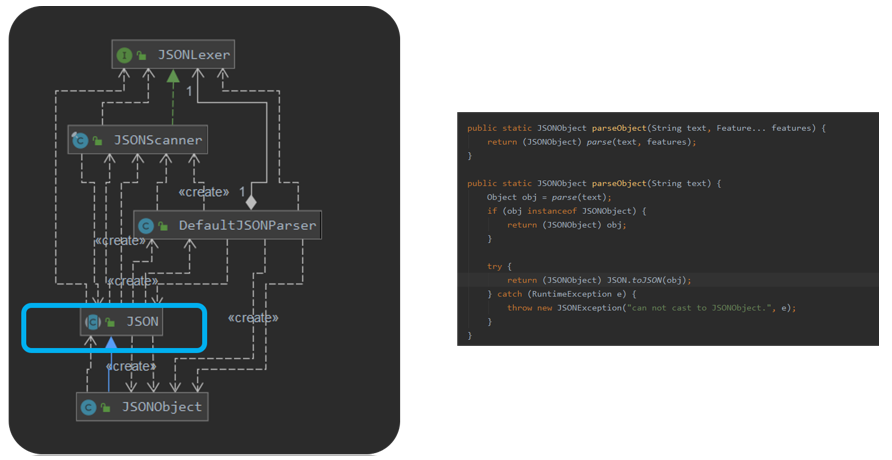
\includegraphics[width = 14cm]{pic9.png}
\caption{Step 1}
\end{figure}

Step2:解析器调用扫描分析器分析词法、寻找键值对
\begin{figure}[H]
\centering % 图片居中
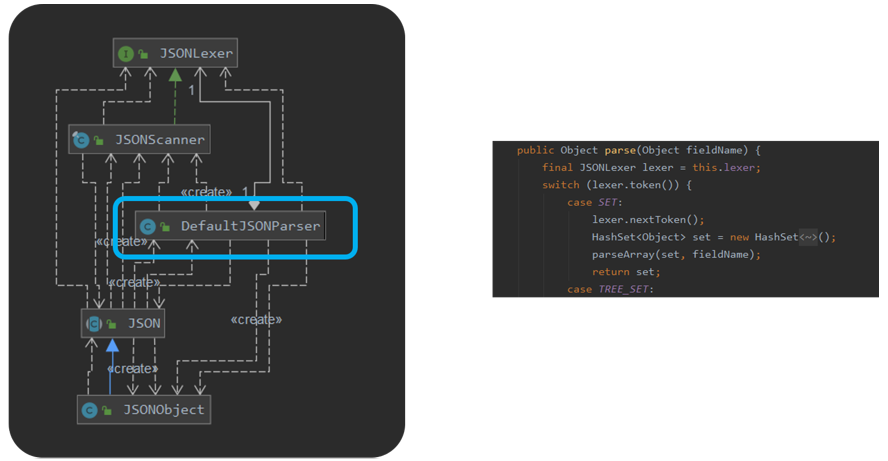
\includegraphics[width = 14cm]{pic10.png}
\caption{Step 2}
\end{figure}

Step3:过程中如果发现输入串非法就报错
\begin{figure}[H]
\centering % 图片居中
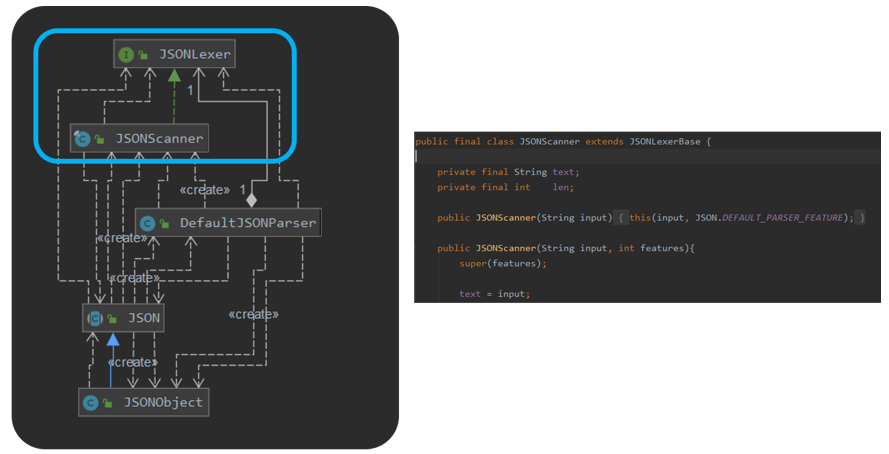
\includegraphics[width = 14cm]{pic11.png}
\caption{Step 3}
\end{figure}

Step4:解析器将结果返回给JAVA对象
\begin{figure}[H]
\centering % 图片居中
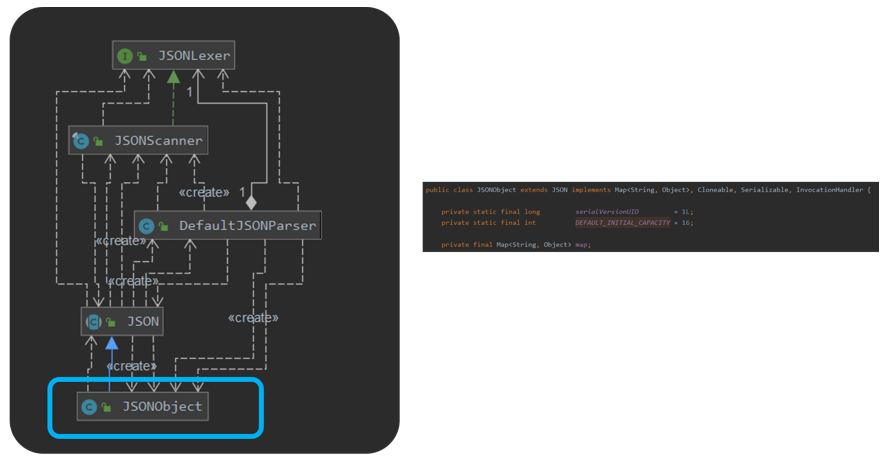
\includegraphics[width = 14cm]{pic12.png}
\caption{Step 4}
\end{figure}

Step5:接口函数返回该JAVA对象: 从JAVA接口中返回,与输入类似,不再附图。

\subsection*{2. UML类图分析}
选取关键模块进行分析:
\begin{figure}[H]
\centering % 图片居中
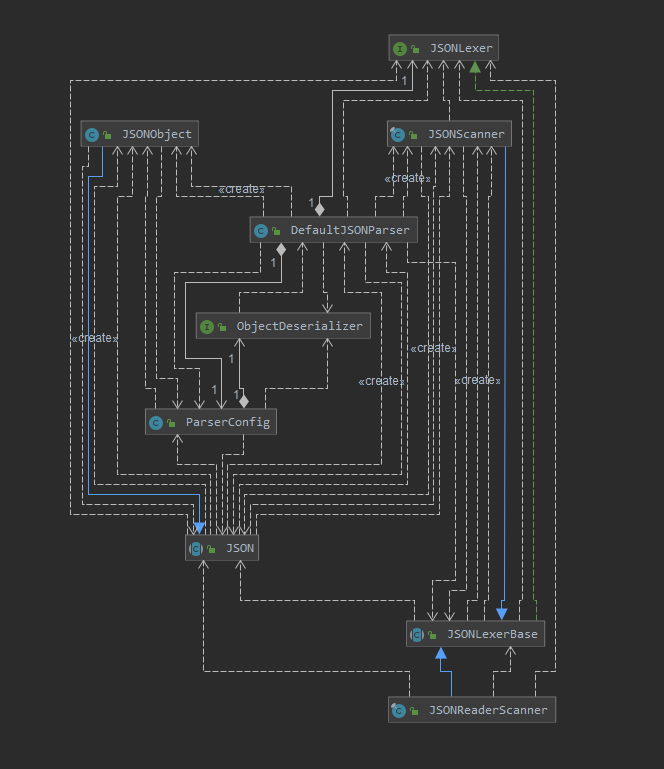
\includegraphics[width = 8cm]{pic13.png}
\caption{UML Class Diagram}
\end{figure}
在我们建模的3个类的基础上,Fastjson额外实现了一些其他的接口和类。下面将对上图中的类一一介绍:
\begin{itemize}
\item JSON抽象类为入口类,它提供了大量的静态方法。
\item JSONObject类继承自JSON抽象类,与我们建模中的用于存储的JAVA对象相对应,存储返回对象。
\item DefaultJSONParser与我们建模中的解析器相对应,依赖于ObjectDeserializer接口、ParserConfig类、JSONObject类、JOSNLexerBase抽象类和JSONLexer接口,并组合到了JSON类上。
\item ObjectDeserializer接口用于提供泛型的支持;ParserConfig类用于处理配置信息。
\item JSONSCanner类和JSONReaderScanner类实现了JSONLexerBase抽象类,该流程中真正被使用的是JSONScanner类,它组合到DefaultJSONParser 类上。
\item 除此之外, JSONException类也相当重要,对应了建模约束中的异常处理,但加入后会使依赖图变得相当混乱,故未标出。
\end{itemize}

\subsection*{3.	UML序列图分析}
参照IntelliJ自动生成的UML序列图(简化前相当复杂)进行简化(只选取建模中所建立的3个类),得到下图:
\begin{figure}[H]
\centering % 图片居中
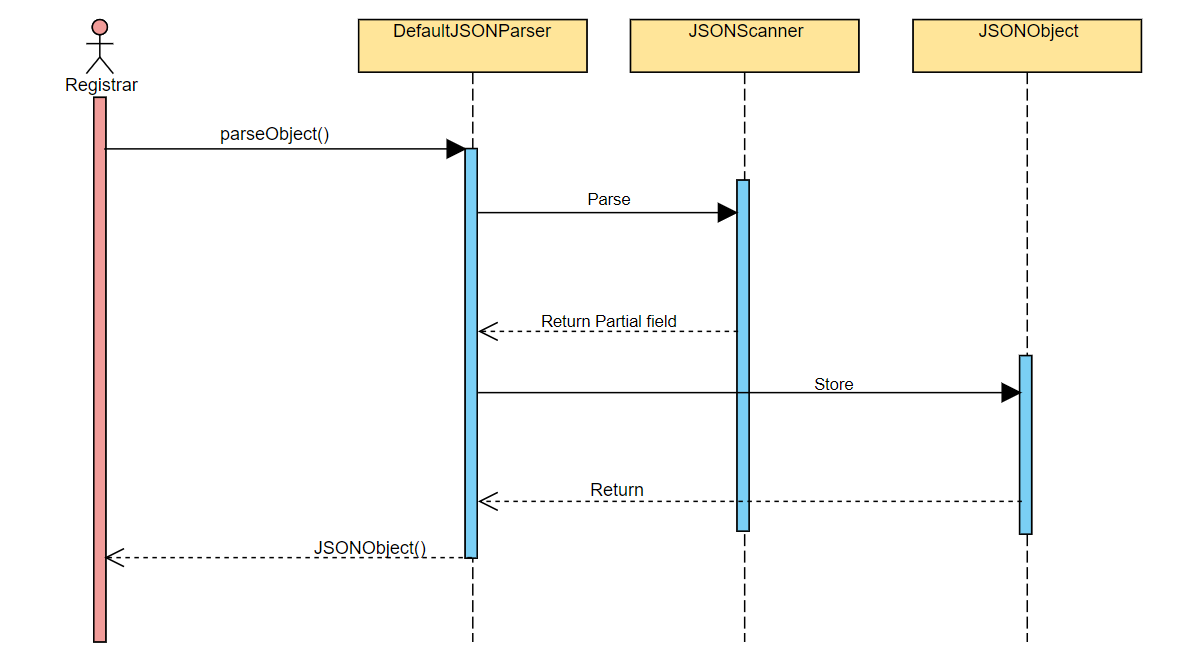
\includegraphics[width = 17cm]{pic14.png}
\caption{UML Sequence Diagram}
\end{figure}
该序列图直接体现了上述建模得到的反序列化流程。


\subsection*{4.	DSM分析}
使用IntelliJ的DSM分析工具对这几个关键的类进行分析,得到下图(位置(m,n)上的数字代表第n列的类多少次依赖于第m行的类):
\begin{figure}[H]
\centering % 图片居中
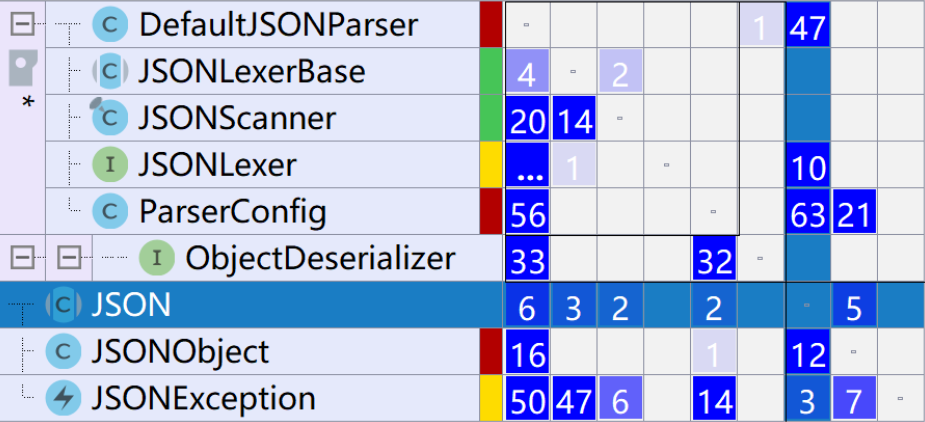
\includegraphics[width = 12cm]{pic15.png}
\caption{Dependency Structure Matrix}
\end{figure}
分析DSM图,可以发现顶层类被底层类大量地依赖,即蓝色区域明显未集中在左下方三角区,可以推断出该项目的类的设置并不是十分合理,有违开闭原则。最明显的体现例如右上角的突兀的47。

\section*{\Large 三、高级设计意图分析}
\subsection*{1.	设计原则}
回顾上一节对重要类的UML类图的分析,与SOLID五大原则对照,能够发现该架构能够体现下述原则:
\subsubsection*{1.1.开闭原则}
\noindent \rule{\textwidth}{0.7mm}
\begin{itemize}
\item 开闭原则(OCP):软件中的对象(类、模块、函数等)应该对于扩展是开放的,但是对于修改是封闭的。
\end{itemize}
\rule{\textwidth}{0.7mm}
JSONLexer接口和JSONLexerBase抽象类的引入使该项目得能够更好地扩展词法分析器,这符合开闭原则。

\subsubsection*{1.2. 合成复用原则}
\noindent \rule{\textwidth}{0.7mm}
\begin{itemize}
\item 合成复用原则(CRP):尽量使用对象组合,而不是继承来达到复用的目的。
\end{itemize}
\rule{\textwidth}{0.7mm}
当一个类要使用另一个类时,代码编写者都尽可能地使用了关联的关系而非继承关系,这是合成复用原则的一个体现。

\subsubsection*{1.3.开闭原则}
\noindent \rule{\textwidth}{0.7mm}
\begin{itemize}
\item 单一职责原则(SRP):就一个类而言,应该仅有一个引起它变化的原因。即一个类中是一组相关性和高的函数,一个类尽量只实现一个功能。
\end{itemize}
\rule{\textwidth}{0.7mm}
该项目在一些地方明显地将复杂的功能拆成小块,从而使得每块都专注于做一件事情。例如:由于词法解析的过程比较复杂,该工能被拆成了词法分析器和解析器两个部分,这体现了单一职责原则。

\subsection*{2. 设计模式}
\subsubsection*{2.1. 策略模式}
\noindent \rule{\textwidth}{0.7mm}
策略模式
\begin{itemize}
\item 意图:定义一系列的算法,把它们一个个封装起来, 并且使它们可相互替换。
\item 主要解决:在有多种算法相似的情况下,使用 if...else 所带来的复杂和难以维护。
\item 何时使用:一个系统有许多许多类,而区分它们的只是他们直接的行为。
\item 如何解决:将这些算法封装成一个一个的类,任意地替换。
\end{itemize}
\rule{\textwidth}{0.7mm}
下图为ObjectDeserializer接口类及其相关部分的实现:
\begin{figure}[H]
\centering % 图片居中
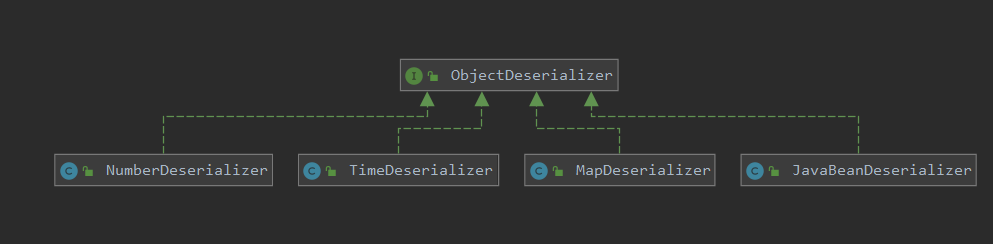
\includegraphics[width = 15cm]{pic16.png}
\caption{About ObjectDeserializer(Class)}
\end{figure}
下图为ObjectDeserializer接口类相关部分的代码:
\begin{figure}[H]
\centering % 图片居中
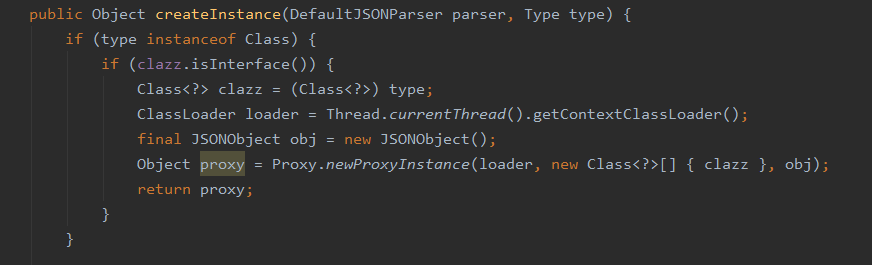
\includegraphics[width = 14cm]{pic17.png}
\caption{About ObjectDeserializer(Code)}
\end{figure}
对照可以发现,ObjectDeserializer接口类中只定义了2个方法,它的子类重写了这两个方法,这就构成了策略模式的一个典型的应用场景。这种方式使得该项目更易增加新的特定类型的反序列化器。

\subsubsection*{2.2. 单例模式}
\noindent \rule{\textwidth}{0.7mm}
单例模式
\begin{itemize}
\item 意图:保证一个类仅有一个实例,并提供一个访问它的全局访问点。
\item 主要解决:一个全局使用的类频繁地创建与销毁。
\item 何时使用:当您想控制实例数目,节省系统资源的时候。
\item 如何解决:判断系统是否已经有这个单例,如果有则返回,如果没有则创建。
\end{itemize}
\rule{\textwidth}{0.7mm}
下图为MapDeserializer类的相关代码:
\begin{figure}[H]
\centering % 图片居中
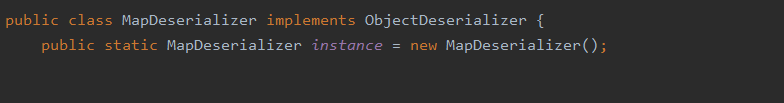
\includegraphics[width = 15cm]{pic18.png}
\caption{About MapDeserializer(Code)}
\end{figure}
该类实现了在类加载时就完成初始化,所以类加载较慢,但获取对象的速度快。这种方式基于类加载机制避免了多线程的同步问题,这是典型的饿汉式的单例模式。这么设计的原因是:当大量反序列化请求同时到达时,Deserilizer会被频繁地创建和销毁,这样会 浪费大量的系统开销。采用单例模式便可以解决该问题,明显降低重复创建和校会的系统开销。

\section*{\Large 四、结语}
终于完成了这份报告,在阅读源码的过程中我学到了很多,自学了java的语法,从实际项目的角度理解了课上讲的一些理论知识,学会了使用IntelliJ来分析项目(真心好用)等等。但由于java水平有限,很多源码都还没有进行仔细分析,毕竟刚接触面向对象编程,要实践的东西还有很多。


在查找资料的过程中,我也发现了一些有趣的事情,发现fastjson虽然速度很快,但使用者的数量似乎依旧比不上gson和jackson,同时可以在各种论坛上找到吐槽fastjson的帖子。在进一步调查后我发现,网友的吐槽大多针对几个方面:其一是fastjson为了提速用了好多“黑科技”,但这些“黑科技”牺牲了整个项目的稳定性和扩展性,而在业界,保证质量过关显然要比提上一点速度重要得多。其二是fastjson的文档和代码比较糟糕,为了求证这一点,我专门对比了gson的英文文档和源码,发现这一点确实无话可说。其三是fastjosn所谓的“快”似乎并没有得到所有人的认同。


这些信息给了我很大的启发,在面向需求建模和编程时,一定要明确各需求间的重要性。比如fastjson宣传的核心就是它的快,可对于企业来说,稳定性可能是更重要的一个部分,至少是不能为了提速牺牲掉的一个部分。以及一定要用心编写文档。


本学期的面向对象程序设计使我受益匪浅,王老师的课别具风格,上课会比较幽默,会结合工业界或者截自己朋友圈的具体的例子来讲解枯燥的概念,所以别具风格。助教哥哥也相当相当友善,QQ上问问题基本都是秒回,实在是太走心了。总的来说,干货很多,相当有诚意。



\end{document}
